\newpage
\section{Особенности строения робота}
Особенности строения использованного в работе робота-машинки (см.~рисунок~\ref{img_robot_gen_view}) даются следующим перечислением:
\begin{itemize}
    \item робот собран из конструктора LEGO Mindstorms EV3;
    \item робот имеет два двигателя со встроенными энкодерами, один из которых (тяговый) приводит в движение задние колеса, а второй (рулевой) поворачивает передние;
    \item усилие с тягового двигателя на задние колеса передается через дифференциал с передаточным отношением, обеспечивающим равенство угловой скорости вращения вала двигателя с полусуммой угловых скоростей задних колес;
    \item рулевые колеса связаны друг с другом и с рулевым двигателем через рулевую трапецию, кинематическая схема которой изображена на рисунке~\ref{img_trapezoid_scheme};
    \begin{figure}[h]
        \centering
        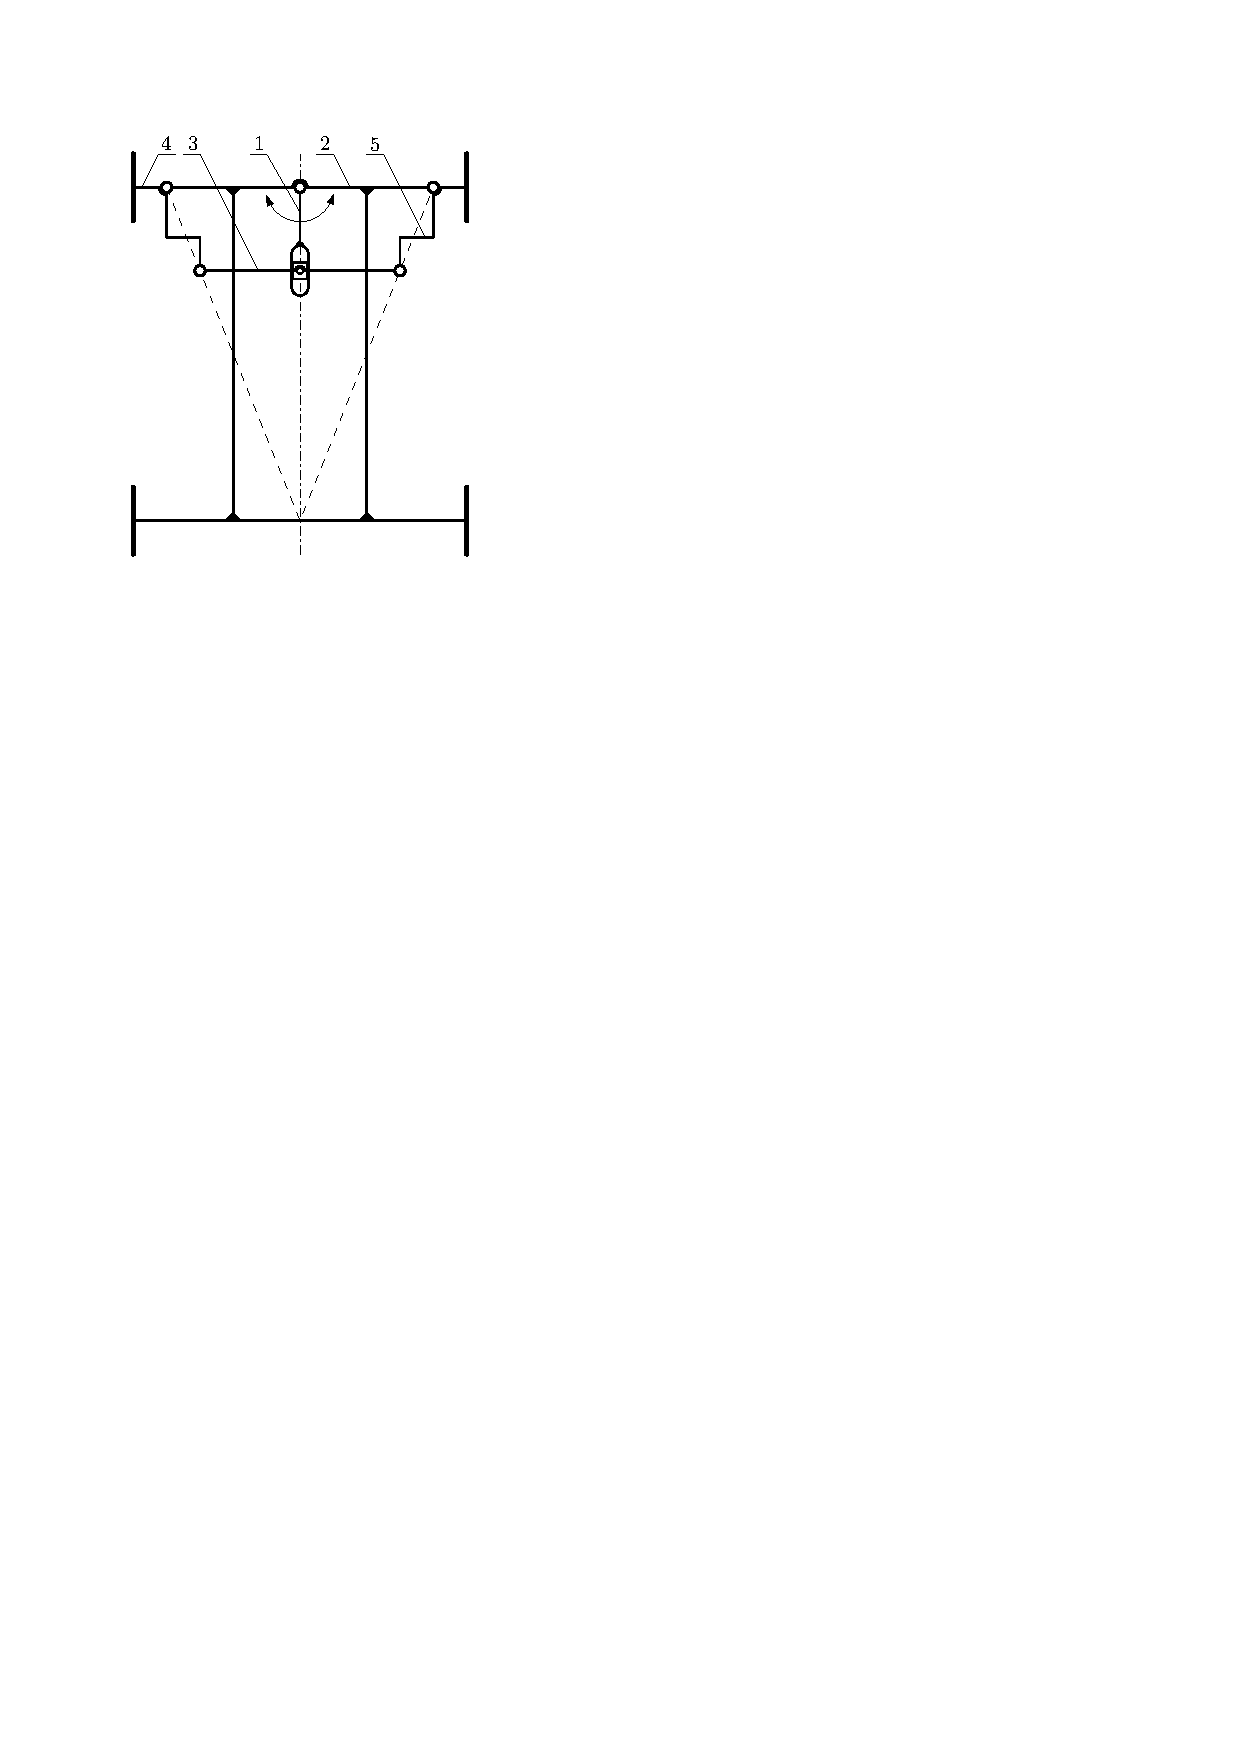
\includegraphics[width= 0.5\textwidth]{trapezoid_kinematic_scheme.pdf}
        \caption{Кинематическая схема рулевой трапеции: 1~--- коромысло, приводимое в движение рулевым двигателем, 2~--- шасси робота, 3~--- шатун, 4,5~--- коромысла, жестко соединенные с осями вращения передних колес.}
        \label{img_trapezoid_scheme}
    \end{figure}
    \item для измерения расстояний до объектов окружающей среды робот имеет два ультразвуковых дальномера;
    \item для определения собственного угла поворота и угловой скорости робот снабжен возвращающим их датчиком-гироскопом.
\end{itemize}

\begin{figure}[h!]
    \begin{minipage}[h]{0.47\textwidth}
        \centering{ \includegraphics[width=\textwidth, draft]{first.jpg} \\ a)}
    \end{minipage}
    \hfill
    \begin{minipage}[h]{0.47\textwidth}
        \centering{ \includegraphics[width=\textwidth, draft]{second.jpg} \\ б)}
    \end{minipage}
    \vfill
    \begin{minipage}[h]{0.47\textwidth}
        \centering{ \includegraphics[width=\textwidth, draft]{third.jpg} \\ в)}
    \end{minipage}
    \hfill
    \begin{minipage}[h]{0.47\textwidth}
        \centering{ \includegraphics[width=\textwidth, draft]{fourth.jpg} \\ г)}
    \end{minipage}
    \caption{Внешний вид использованного в работе робота-машинки.}
    \label{img_robot_gen_view}
\end{figure}

\newpage
\mbox{}
